\documentclass[a4paper, 14pt]{extreport}
\usepackage[T2A]{fontenc}
\usepackage[utf8]{inputenc}
\usepackage[english, russian]{babel}
\usepackage{indentfirst, setspace, titlesec, subcaption}
\usepackage{hyperref}
\usepackage{graphicx}
\usepackage{tocloft}
\usepackage{multirow}
\usepackage[left=2.5cm, right=1.5cm, top=2.0cm, bottom=2.0cm]{geometry}

\usepackage{array}
\newcolumntype{C}[1]{>{\centering\arraybackslash}m{#1\textwidth}}
\renewcommand{\arraystretch}{1.2}

\graphicspath{{images/}}
\renewcommand{\rmdefault}{ftm}

\titleformat{\chapter}
    {\normalsize}
    {\thechapter}{1em}{}
\titleformat{\section}
    {\normalsize}
    {\thesection}{1em}{}
\titlespacing*{\chapter}{\parindent}{-30pt}{*2}
\titlespacing*{\paragraph}{\parindent}{-30pt}{*2}
\titlespacing*{\section}{\parindent}{*2}{*2}

\renewcommand{\cfttoctitlefont}{\normalfont\hspace{0.38\textwidth}}
\renewcommand{\cftchapleader}{\cftdotfill{\cftdotsep}}
\renewcommand{\cftbeforepartskip}{0em}
\renewcommand{\cftbeforechapskip}{0em}
\renewcommand{\cftchapfont}{\hspace{15pt}\normalsize}
\renewcommand{\cftsecfont}{\hspace{-6pt}}
\renewcommand{\cftsubsecfont}{\hspace{-38pt}}
\renewcommand{\cftchappagefont}{\normalfont}
\renewcommand{\cftbeforetoctitleskip}{-1em}
\renewcommand{\cftpartaftersnumb}{}
\renewcommand{\cftparskip}{-1mm}
\renewcommand{\cftdotsep}{2}

\begin{document}
    \begin{titlepage}
        \begin{center}
            Министерство образования и науки РФ \\
            Государственное образовательное учреждение\\
            Высшего профессионального образования\\
            <<Волгоградский государственный технический университет>>\\
            Кафедра <<САПР~и~ПК>>
        \end{center}
        \vspace{2.0cm}
        \begin{center}
            \large \textbf{ОТЧЕТ} \\
            по преддипломной практике \the\year г.
        \end{center}
        \begin{flushleft}
            Студента\\
            Фамилия \underline{Чечеткина\hspace{2.825cm}} 
            Имя \underline{Ильи\hspace{2.7cm}}\\
            Отчество \underline{Александровича\hspace{1.5cm}}\\
            Факультет \underline{ФЭВТ\hspace{3.45cm}} курс \underline{2\hspace{1.5cm}} 
            группа \underline{САПР-2.1п\hspace{1.9cm}}\\
        \end{flushleft}
        \vspace{1.0cm}
        \noindentИндивидуальное задание: \underline{\hspace{22.3em}}\\
        \underline{\hspace{\textwidth}}
        \underline{\hspace{\textwidth}}
        \underline{\hspace{\textwidth}}
        \underline{\hspace{\textwidth}}
        \vspace{2.0cm}
        \begin{flushleft}
            РУКОВОДИТЕЛЬ\\
            Кафедра \underline{САПР~и~ПК\hspace{2.4cm}} Должность \underline{профессор\hspace{2.8cm}} \\
            Фамилия \underline{Кравец\hspace{3.3cm}} Имя \underline{Алла\hspace{5.5cm}}\\
            Отчество \underline{Григорьевна\hspace{2.2cm}}
        \end{flushleft}
        \vspace{1.5cm}
        \begin{flushright}
            <<\underline{\hspace{1.0cm}}>>\underline{\hspace{4.0cm}} \the\year г.
        \end{flushright}
        \vspace{\fill}
        \begin{center}
            Волгоград \the\year
        \end{center}
    \end{titlepage}
    \tableofcontents
    \onehalfspacing

    \chapter{Методика тестирования системы кластеризации}
    Алгоритмы, предложенные в рамках магистерской работы, были реализованы с использованием языка программирования Python и сервиса построения маршрутов Open Source Routing Machine для расчета расстояния между узлами графа по городским дорогам. Программный код опубликован на хостинге Github 
    \url{https://github.com/vstu-cad-stuff/clustering/tree/master}.

    Для оценки эффективности работы алгоритма и изучения специфики разработанной метрики были проведены эксперименты, в ходе которых менялись выборки данных, количество получаемых кластеров и их начальное местоположение, а так же реализация метода.

Для оценки работы алгоритма на данных, приближенных к реальным, были сгенерированы данные о предпочтениях по перемещению жителей среднего по размерам города с примерным числом жителей около 350 000. В качестве результата было получено 6000 пар точек отправления--назначения (рис.~\ref{pic:full}), или 12000 точек в общей сложности (выборка Main). Эту выборку было решено разбить на 125 кластеров, начальное положение которых было случайным. В последствие это случайное расположение кластеров было взято за основу для тестирования различных версий алгоритма.

\begin{figure}[ht!]
    \centering
    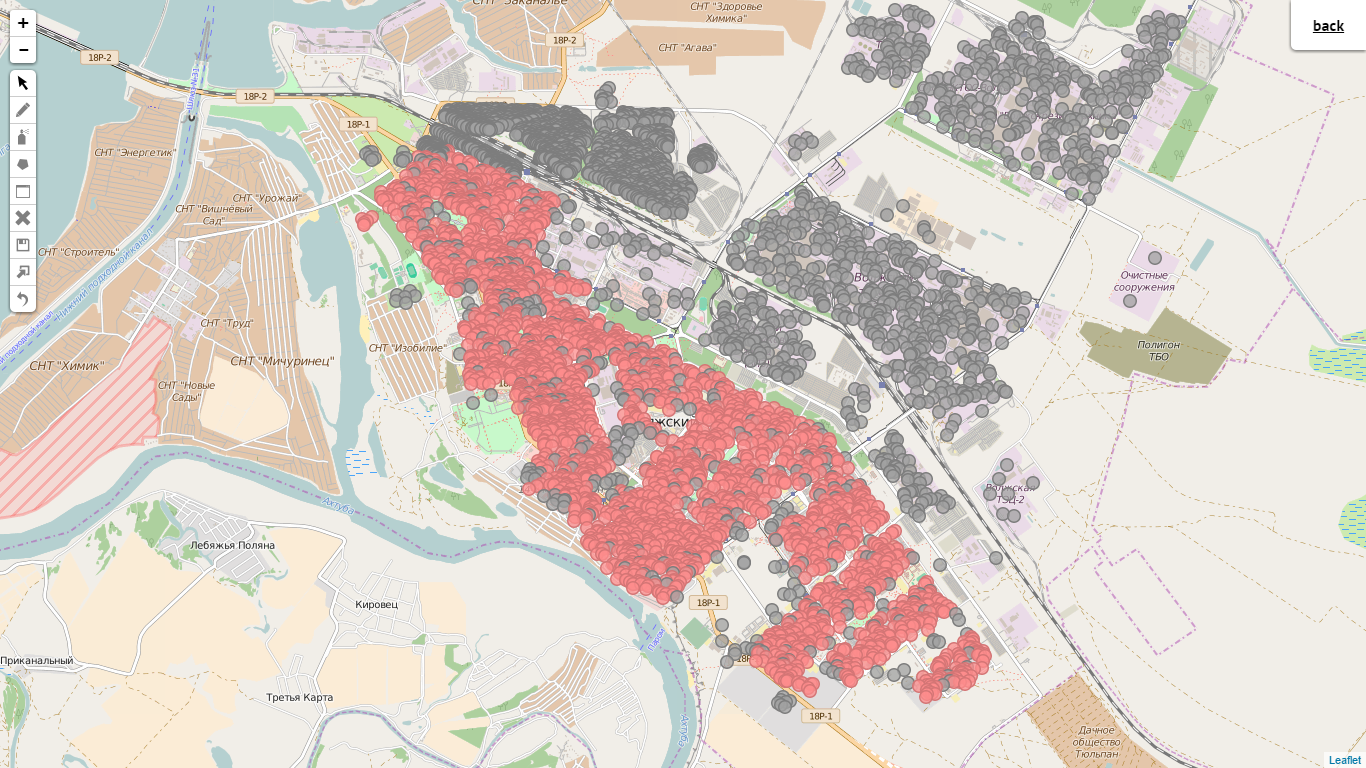
\includegraphics[width=.9\textwidth]{full} \\[1ex]
    \parbox{.9\textwidth}{\caption{Сгенерированная выборка из 12000 точек. Красным отмечены точки отправления, серым~--- назначения} \label{pic:full}}
    \vspace*{-1ex}
\end{figure}

\begin{figure}[t!]
    \centering
    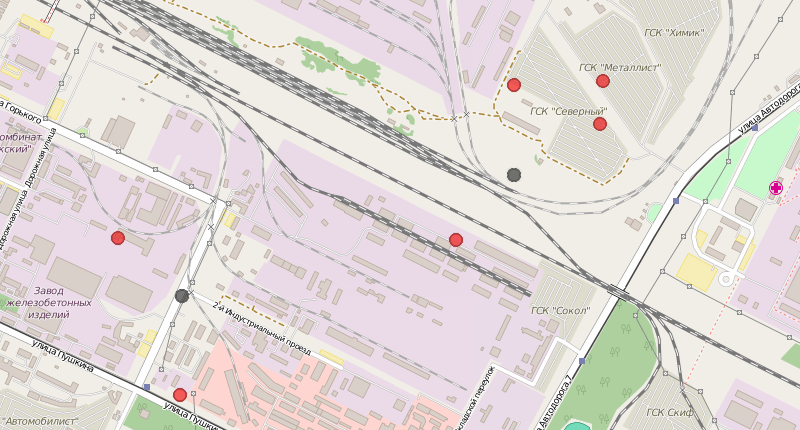
\includegraphics[width=.47\textwidth]{test_railway-contrast}\
    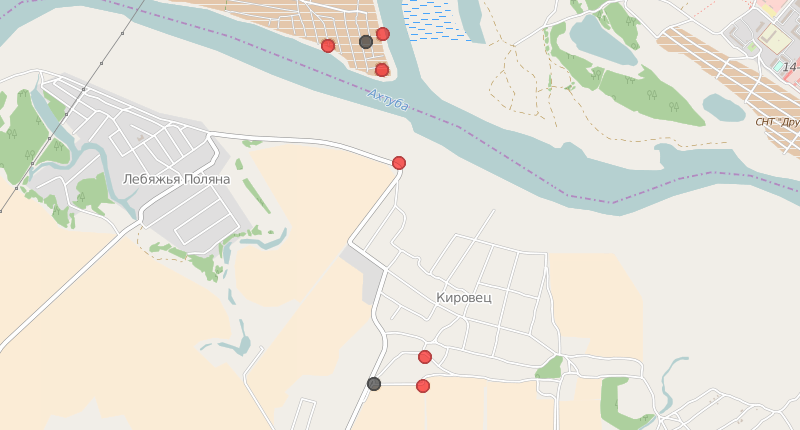
\includegraphics[width=.47\textwidth]{test_river-contrast} \\
    \parbox{.47\textwidth}{\small\centering a)}\ \parbox{.47\textwidth}{\small\centering б)}
    \parbox{.9\textwidth}{\caption{Выборки для проверки обхода препятствий. На рисунке а) между объектами выборки находится железная дорога, на рисунке б)~--- река. Красными кругами отмечены элементы выборки, черными~--- начальные центры кластеров} \label{pic:railway-river}}
    \vspace*{-1ex}
\end{figure}

Так же были сгенерированы другие выборки для проверки специфичных случаев: обхода препятствий в виде железной дороги (выборка Railway, рис.~\ref{pic:railway-river}а) и реки (выборка River, рис.~\ref{pic:railway-river}б). Каждая из них представляет собой набор из шести точек, которые кластеризуются в два кластера. Точки и начальные центры расположены таким образом, что если алгоритм не учитывает препятствия между объектами выборки, то в одном кластере окажутся точки, разделенные препятствием.

Критериями для оценки эффективности разработанных алгоритмов и метрик являются:
\begin{itemize}
    \item время, затраченное на расчет расстояния между объектами выборки;
    \item учет препятствий;
    \item визуальная оценка результатов кластеризации.
\end{itemize}

    \chapter{Произведение испытаний разработанной системы}
    Для тестирования эффективности работы алгоритма была использована еще одна выборка, представленная на рисунке~\ref{pic:common}.
\begin{figure}[h!]
    \centering
    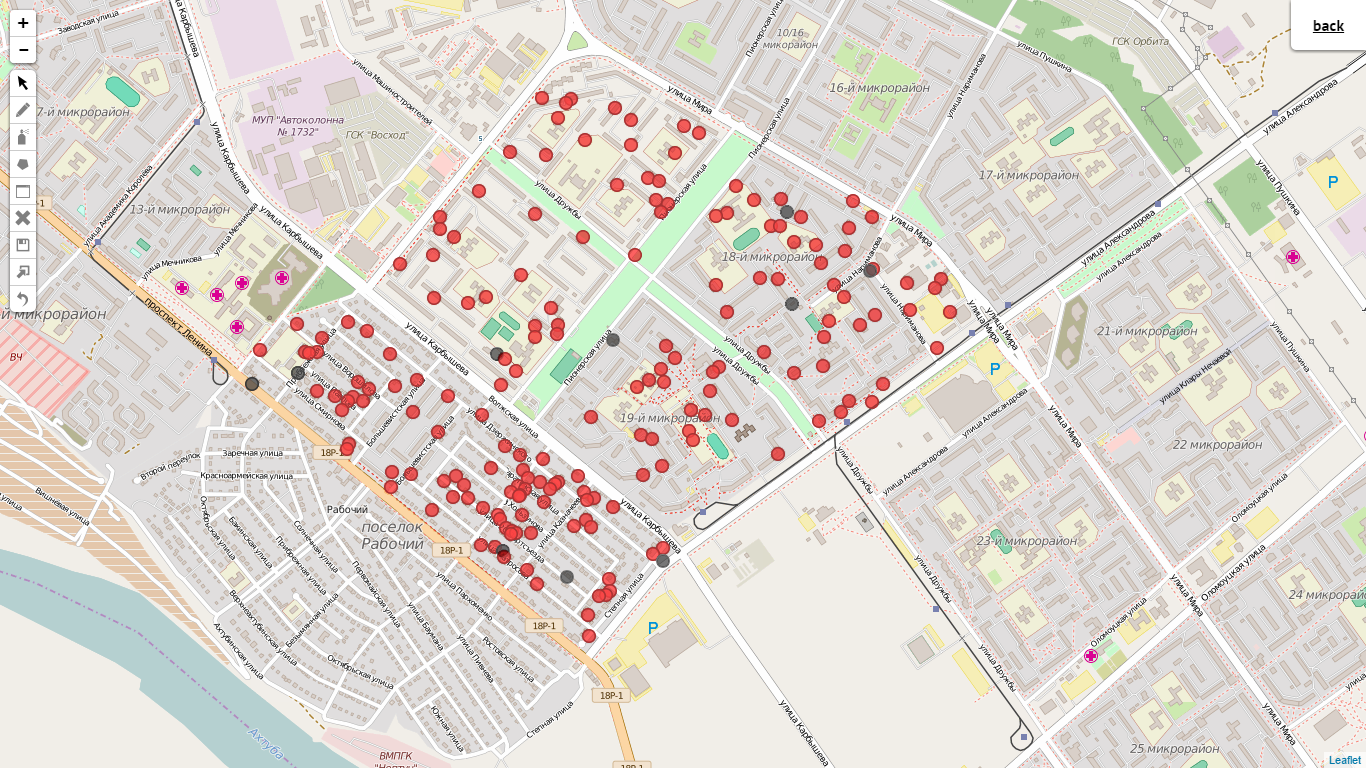
\includegraphics[width=.7\textwidth]{test_common-contrast}\\[1ex]
    \parbox{.9\textwidth}{\caption{Выборка Common. Красными кругами отмечены элементы выборки, черными~--- начальные центры кластеров}\label{pic:common}}
\end{figure}
    
    Таким образом, для тестирования работы алгоритма было использовано 4 выборки:
\begin{itemize}
    \item выборка Main: \( |X| = 12 000 \) точек, \( k = 125 \) (рис.~\ref{pic:full}); используется для общего тестирования работы алгоритмов;
    \item выборка Railway: \( |X| = 6 \) точек, \( k = 2 \) (рис.~\ref{pic:railway-river}а); используется для проверки обхода препятствий;
    \item выборка River: \( |X| = 6 \) точек, \( k = 2 \) (рис.~\ref{pic:railway-river}б); используется для проверки обхода препятствий;
    \item выборка Common: \( |X| = 180 \) точек, \( k = 10 \) (рис.~\ref{pic:common}); используется для тестов алгоритмов на скорость.
\end{itemize}

    Чтобы понять эффективность работы алгоритма в зависимости от окружающей среды, были разработаны три альтернативных 
    реализации:
    \begin{enumerate}
        \item Последовательная реализация алгоритма, расчитывающего расстояние между объектами по прямой, не учитывая препятствия между ними (метрика Surface). Эту реализацию можно рассматривать в качестве базовой.
        \item Последовательная реализация с использованием OSRM~--- это усовершенствованная версия 
            предыдущей стратегии, где расстояние между объектами рассчитывается с использованием движка 
            маршрутизации OSRM по дорожной сети (метрика Route).
        \item Параллельная версия с использованием OSRM предполагает возможность в распараллеливании внутреннего цикла алгоритма.  
    \end{enumerate}

    \chapter{Результаты полученные в входе работы}
    Результаты кластеризации выборок Railway и River для обоих метрик представлены на рисунках \ref{pic:test_surface_results} и \ref{pic:test_route_results}.

\begin{figure}[h!]
    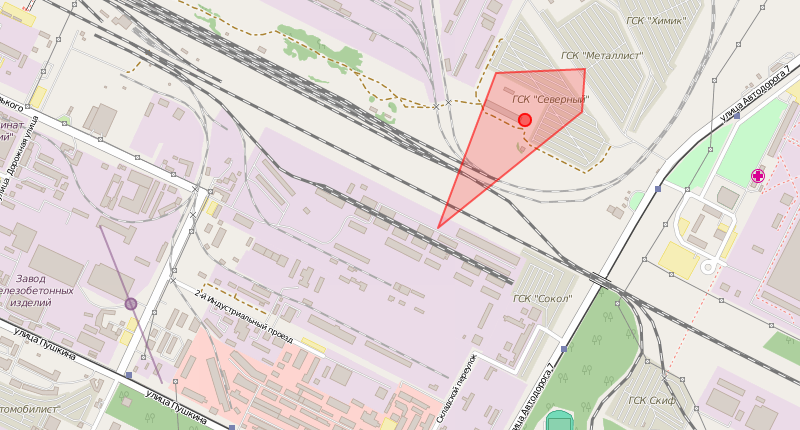
\includegraphics[width=.47\textwidth]{railway_surface}\
    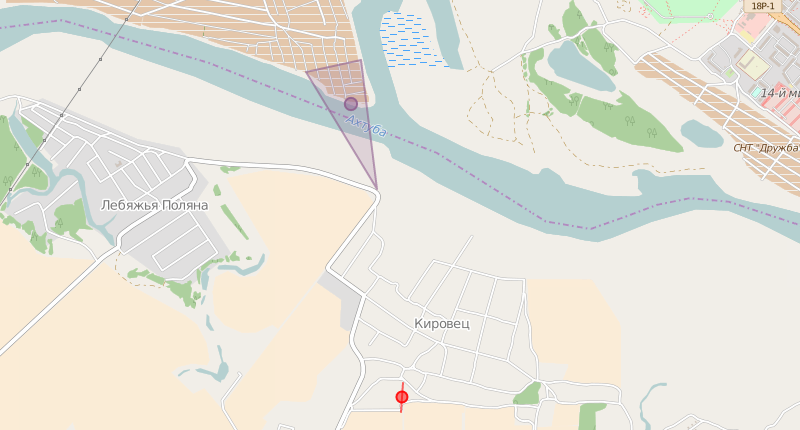
\includegraphics[width=.47\textwidth]{river_surface} \\[1ex]
    \parbox{.95\textwidth}{\caption{Результаты кластеризации выборок Railway и River с метрикой Surface}\label{pic:test_surface_results}}
    \vspace*{-3ex}
\end{figure}

\begin{figure}[h!]
    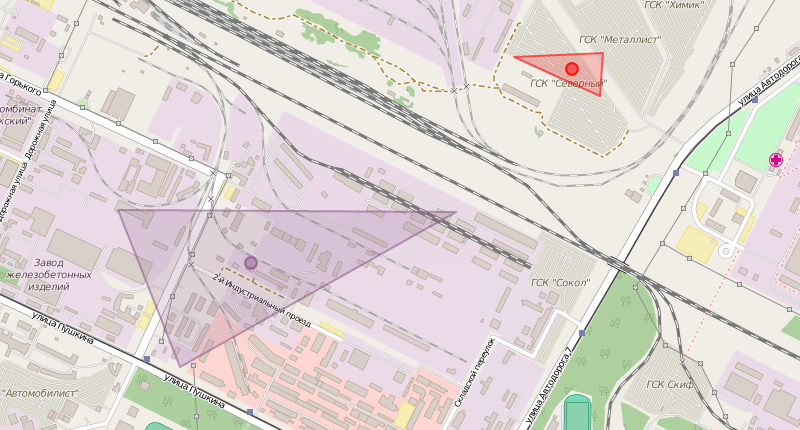
\includegraphics[width=.47\textwidth]{railway_route}\
    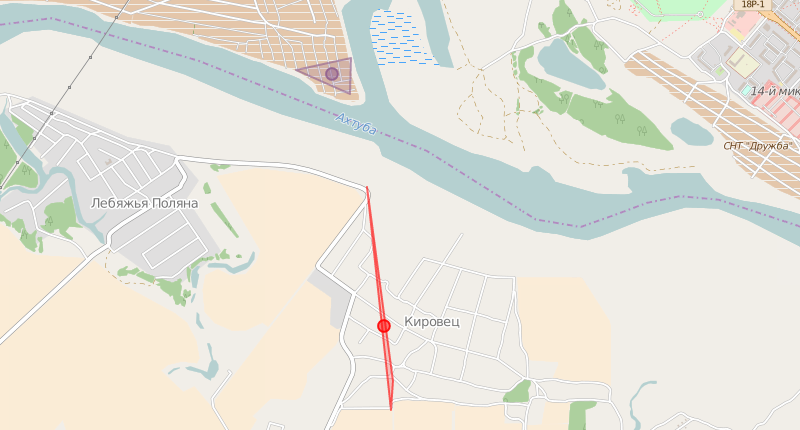
\includegraphics[width=.47\textwidth]{river_route} \\[1ex]
    \parbox{.95\textwidth}{\caption{Результаты кластеризации выборок Railway и River с метрикой Route}\label{pic:test_route_results}}
    \vspace*{-2ex}
\end{figure}
Результаты обработки выборки Main представлены на рисунках~\ref{pic:full-surface}, \ref{pic:full-route}.

В таблице~\ref{tab:results} приведены средние длительности выполнения одного расчета дистанции между геопространственными объектами для трех реализаций алгоритма: последовательной, параллельной на два потока и параллельной на 4 потока, и для трех метрик: Euclid, Surface и Route. Метрика Euclid является обычной евклидовой метрикой: \( \rho(a, b) = \sqrt{(a.x - b.x)^2 + (a.y - b.y)^2} \) и приводится для сравнения. Величины приведены в миллисекундах.

\begin{table}[b!]
    \vspace*{-10em}
    \caption{Среднее время выполнения одного расчета расстояния при различных метриках и реализациях алгоритма, мс}
    \label{tab:results}
    \centering
    \begin{tabular}{|l|*{3}{C{.15}|}} \hline
        Реализация       & Euclid & Surface & Route \\ \hline
        Последовательная & 0,0665 &  0,709  & 4,785 \\ \hline
        Параллельная (2) & 0,0659 &  0,692  & 4,069 \\ \hline
        Параллельная (4) & 0,0654 &  0,663  & 3,596 \\ \hline
    \end{tabular}
\end{table}

\newpage

\begin{figure}[t!]
    \vspace{-10em}
    \centering
    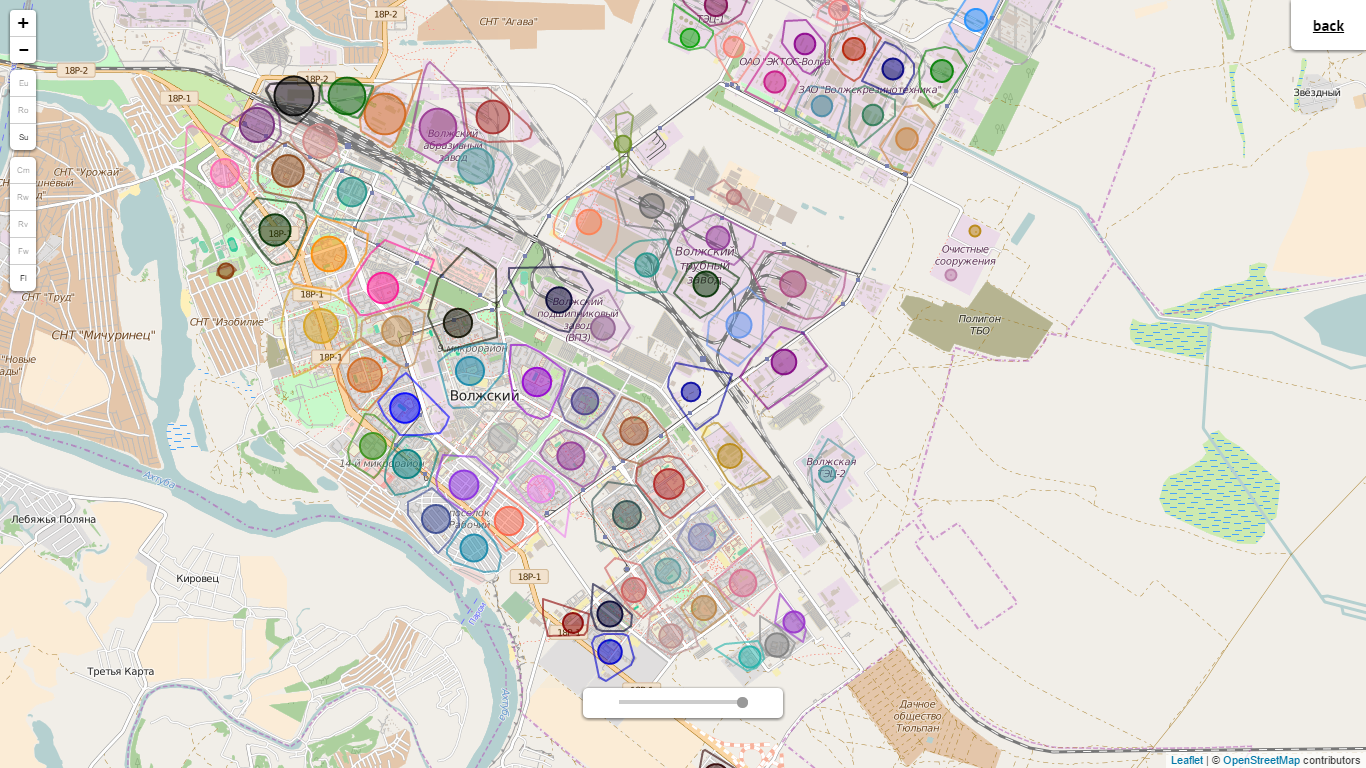
\includegraphics[width=.95\textwidth]{full_surface}\\[1ex]
    \parbox{.95\textwidth}{\caption{Результаты обработки выборки Main метрикой Surface}\label{pic:full-surface}}
    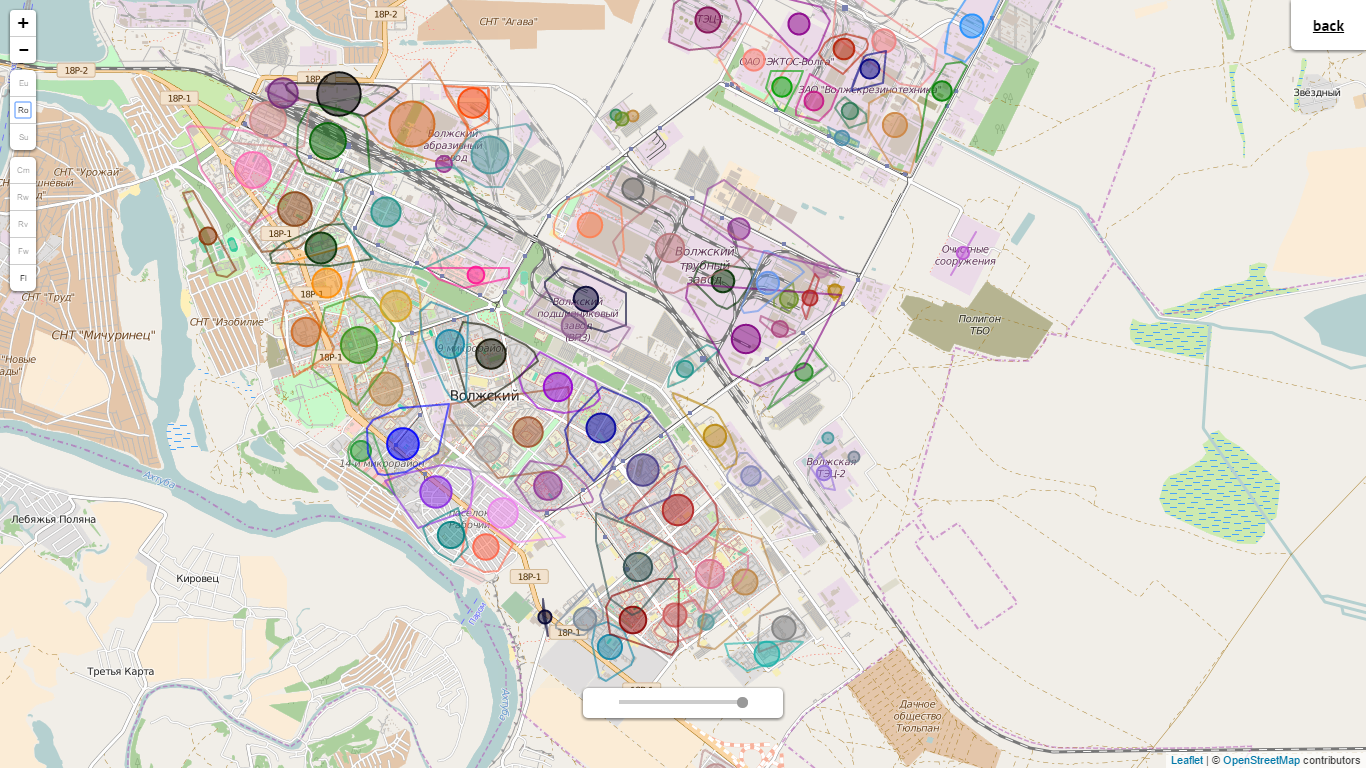
\includegraphics[width=.95\textwidth]{full_route}\\[1ex]
    \parbox{.95\textwidth}{\caption{Результаты обработки выборки Main метрикой Route}\label{pic:full-route}}
\end{figure}

    \chapter{Структура четвертой главы магистерской диссертации}
    В структуре четвертой главый магистерской диссертации были выделены следующие пункты:
    \begin{enumerate}
        \item Испытание и обоснование эффективности предлагаемых подходов
        \begin{enumerate}
            \item Проектирование ПО
            \item Методика проведения эксперимента
        \end{enumerate}
        \item Описание результатов испытания
        \begin{enumerate}
            \item Проведение эксперимента и описание результатов
            \begin{enumerate}
                \item Последовательная реализация
                \item Последовательная с использованием OSRM
                \item Параллельная с использованием OSRM
                \item Результаты
            \end{enumerate}
            \item Обсуждение результатов
            \item Выводы
        \end{enumerate}
    \end{enumerate}

    В разделе <<Испытание и обоснование эффективности предлагаемых подходов>> описана методика тестирования 
    разработанных алгоритмов и данные используемые для проведения тестирования.

    В разделе <<Описание результатов испытания>> были предложены три альтернативных реализации алгоритма для оценки его 
    эффективности в зависимости от входных данных. В данном разделе производится оценка эффективности альтернативных 
    реализаций и их общее сравнение. Результатом работы являются визуализации работы данных реализаций, представленные 
    на рисунках \ref{pic:full-surface} и \ref{pic:full-route}, а также данные в таблице \ref{tab:results}.

    \chapter{Выводы по проделанной работе}
    В ходе преддипломной практики были выполнены следующие задачи:
    \begin{itemize}
        \item разработана методика тестирования системы кластеризации геораспределенных данных;
        \item произведены испытания разработанной системы на тестовом наборе входных данных;
        \item произведена оценка разработанной системы и обоснована эффективность 
                используемых алгоритмов.
    \end{itemize}

    \chapter{Используемые технологии в работе}
    Для проектирования и верстки были использованы следующие свободно распространяемые программные 
    продукты:
    \begin{itemize}
        \item Linux Mint -- это i686/x86-64 дистрибутив GNU/Linux общего 
            назначения, разрабатываемый на основе Ubuntu/Debian.\\
            \url{https://www.linuxmint.com/}
        \item \TeX -- система компьютерной верстки, разработанная американским профессором информатики 
            Дональдом Кнутом в целях создания компьютерной типографии.
            \hspace{1ex} \url{http://tug.org/}
        \item \LaTeX -- набор макрорасширений системы компьютерной верстки TeX.\\
            \url{http://www.latex-project.org/}
        \item Atom -- свободный открытый текстовой редактор исходных текстов программ.
            \hspace{1ex} \url{https://atom.io/}
        \item Python -- высокоуровневый язык программирования общего назначения, ориентированный на повышение 
            производительности разработчика и читаемости кода.
            \hspace{1ex} \url{https://www.python.org/}
        \item Leaflet -- Open-Source библиотека, предназначенная для отображения         карт на веб-сайтах.
            \hspace{1ex} \url{http://leafletjs.com/}
        \item Git -- распределенная система управления версиями файлов. Проект был создан Линусом 
            Торвальдсом для управления разработкой ядра Linux, первая версия выпущена 7 апреля 2005 года.\\
            \url{http://git-scm.com/}
        \item GitHub -- самый крупный веб-сервис для хостинга IT-проектов и их совместной разработки. 
            Основан на системе контроля версий Git и разработан на Ruby on Rails и Erlang компанией 
            GitHub, Inc.\\ \url{https://github.com/}
    \end{itemize}
\end{document}